% LaTeX Template for short student reports.
% Citations should be in bibtex format and go in references.bib
\documentclass[a4paper, 11pt]{article}
\usepackage[top=3cm, bottom=3cm, left = 2cm, right = 2cm]{geometry} 
\geometry{a4paper} 
\usepackage[utf8]{inputenc}
\usepackage{textcomp}
\usepackage{graphicx} 
\usepackage{mathtools}
\usepackage{diffcoeff}
\usepackage{amsmath,amssymb}  
\usepackage{bm}  
\usepackage[pdftex,bookmarks,colorlinks,breaklinks]{hyperref}  
%\hypersetup{linkcolor=black,citecolor=black,filecolor=black,urlcolor=black} % black links, for printed output
\usepackage{memhfixc} 
\usepackage{pdfsync}  
\usepackage{fancyhdr}
\usepackage{movie15}
\pagestyle{fancy}

\title{DBSCAN Report}
\author{Donal Loitam}
%\date{}

\begin{document}
\maketitle
\tableofcontents

\section{Introduction}
\begin{itemize}
    \item \textbf{Clusters} are dense regions in the data space, separated by regions of the lower density of points
    \item  The \textbf{DBSCAN(Density-based spatial clustering of applications with noise) algorithm} is based on this intuitive notion of \textbf{“clusters”} and \textbf{“noise”}.
    \item The key idea is that for each point of a cluster, the neighborhood of a given radius has to contain at least a minimum number of points. 
\end{itemize}
\begin{figure}[h!]
    \centering
    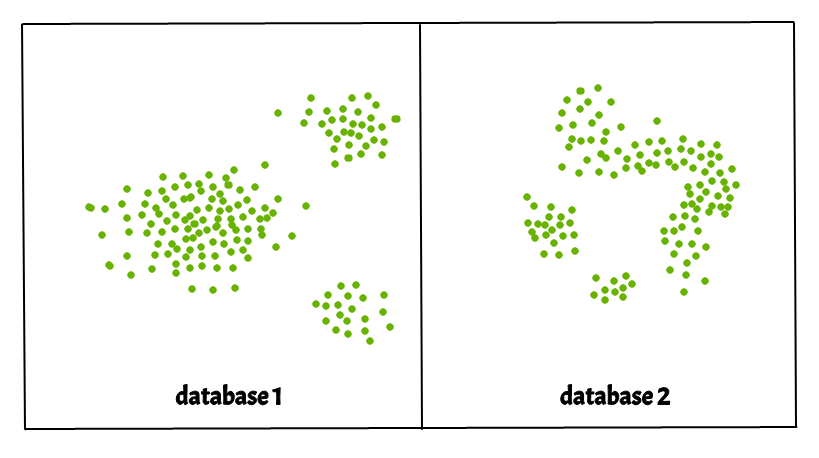
\includegraphics[width=0.45\linewidth]{d1.png}
    \label{fig:fig1}
  \end{figure}

\section{The Problem with k-Means Clustering :}
\begin{itemize}
    \item Partitioning methods (K-means) work for finding spherical-shaped clusters or convex clusters i.e they are suitable only for compact and well-separated clusters
    \item Moreover, they are also severely affected by the presence of noise and outliers in the data.
    \item And as we know, \textbf{Real life data often contain irregularities and noise}
\end{itemize}

\section{Key Points of the Algorithm}
\begin{itemize}
    \item \textbf{Parameters of DBSCAN algorithm:}
      \begin{enumerate}
       \item \textbf{eps :} It defines the neighborhood around a data point i.e. if the distance between two points is lower or equal to ‘eps’ then they are considered neighbors. If the eps value is chosen too small then large part of the data will be considered as outliers. If it is chosen very large then the clusters will merge and the majority of the data points will be in the same clusters. One way to find the eps value is based on the k-distance graph.
       \item \textbf{MinPts: } Minimum number of neighbors (data points) within eps radius. Larger the dataset, the larger value of MinPts must be chosen. As a general rule, the minimum MinPts can be derived from the number of dimensions D in the dataset as, MinPts >= D+1. The minimum value of MinPts must be chosen at least 3.
      \end{enumerate}

    \item \textbf{3 types of Datapoints in the algorithm}:
    \begin{enumerate}
        \item \textbf{Core Point:} A point is a core point if it has \textbf{more than MinPts points} within eps radius 
        \item \textbf{Border Point:} A point which has fewer than MinPts within eps but it is in the neighborhood of a core point. 
        \item \textbf{Noise or outlier:} A point which is not a core point or border point.

        \item Below is a figure depicting the three types of datapoints and the parameters of the algorithm
        \begin{figure}[ht!]
          \centering
          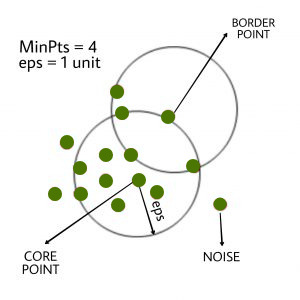
\includegraphics[width=0.45\linewidth]{d2.jpeg}
          \caption{figure depicting types of datapoints and parameters involved}
          \label{fig:fig2}
        \end{figure}    
    \end{enumerate}
    \item  \textbf{The Algorithm at a Glance: }
    \begin{enumerate}
        \item Find all the neighbour points within eps and \textbf{identify the core points} or visited with more than MinPts neighbors.
        \begin{figure}[ht!]
          \centering
          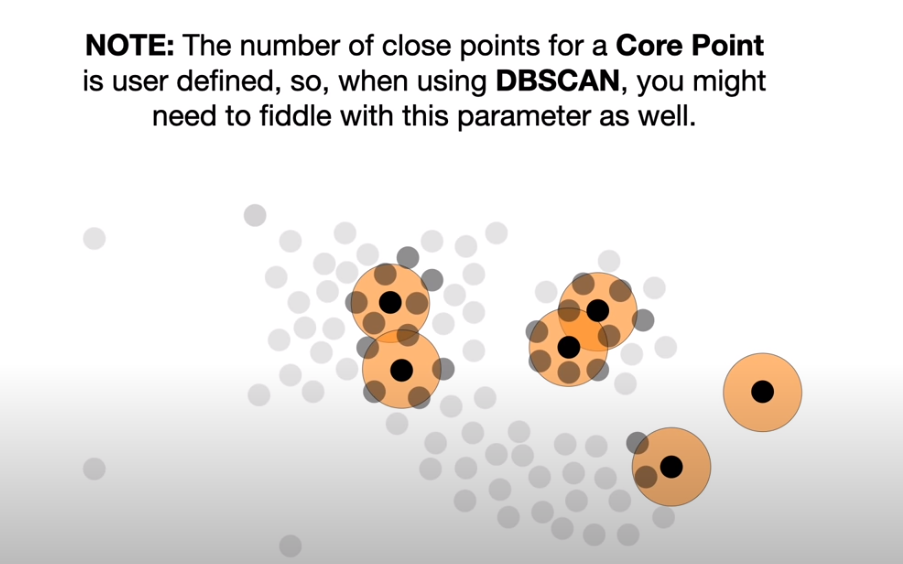
\includegraphics[width=0.45\linewidth]{ss1.png}
          \caption{\textbf{MinPts is userdefined, here MinPts=4}}
          \label{fig:fig3}
        \end{figure}\\
        \item \textbf{For each core point}, if it is not already assigned to a cluster, \textbf{create a new cluster.}\\
        \begin{figure}[ht!]
          \centering
          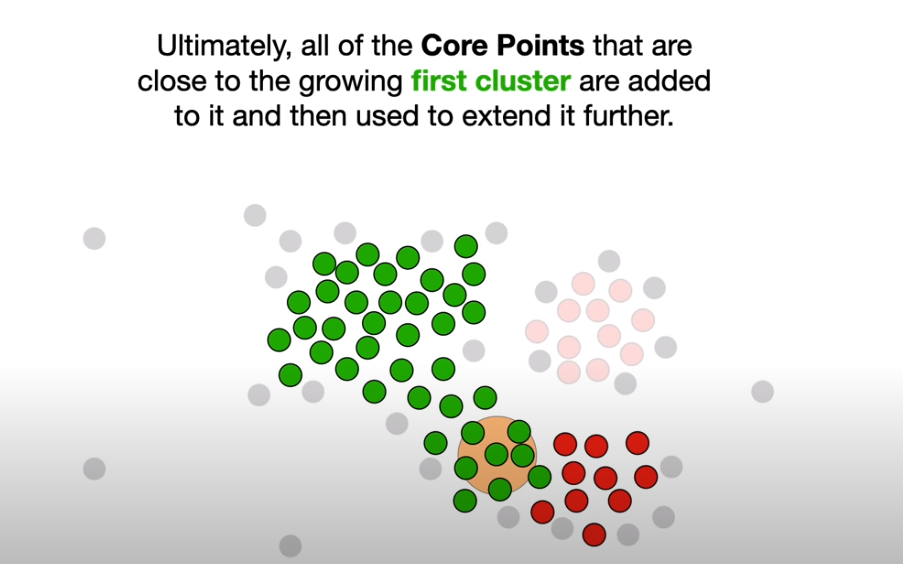
\includegraphics[width=0.45\linewidth]{ss2.png}
          \caption{\textbf{Creating a cluster}}
          \label{fig:fig4}
        \end{figure}
        \item Find recursively all its density connected points and assign them to the same cluster as the core point. 
        
        A point a and b are said to be density connected if there exist a point c which has a sufficient number of points in its neighbors and both the points a and b are within the eps distance. This is a chaining process. So, if b is neighbor of c, c is neighbor of d, d is neighbor of e, which in turn is neighbor of a implies that b is neighbor of a.
        \begin{figure}[ht!]
          \centering
          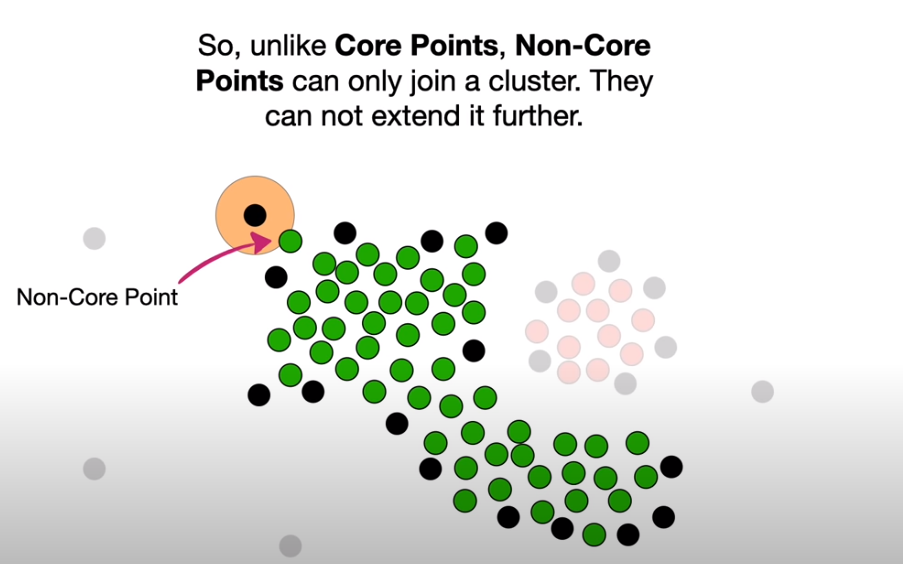
\includegraphics[width=0.445\linewidth]{ss4.png}
          \caption{\textbf{Assigning Clusters to Non-Core points}}
          \label{fig:fig5}
        \end{figure}
        \item Iterate through the remaining unvisited points in the dataset. Those points that do not belong to any cluster are \textbf{noise.}
        \begin{figure}[ht!]
          \centering
          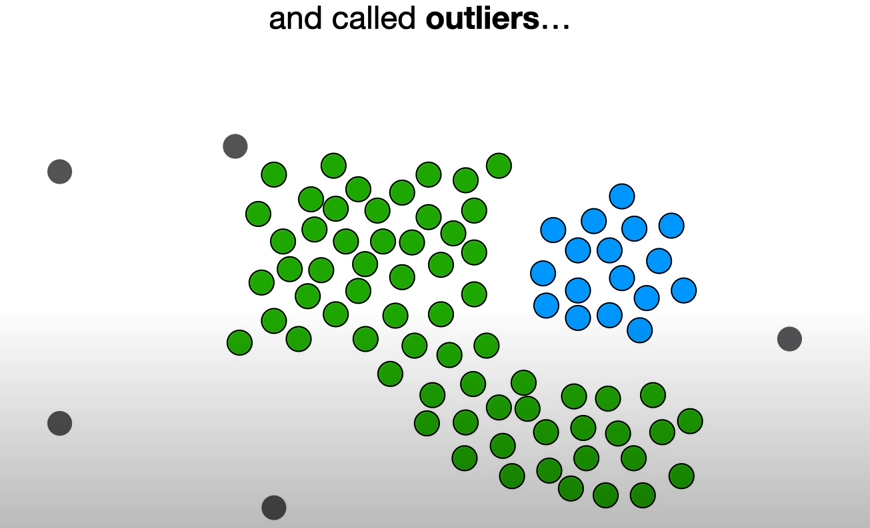
\includegraphics[width=0.445\linewidth]{ss6.png}
          \caption{\textbf{Black points which are not near are called noise/outliers}}
          \label{fig:fig6}
        \end{figure}
    \end{enumerate}  
    \item \textbf{DBSCAN clustering algorithm in pseudocode:}\\
    DBSCAN(dataset, eps, MinPts)\{\\
   \#cluster index\\
   C = 1 \\
   for each unvisited point p in dataset  \{ \\
        mark p as visited \\
        \# find neighbors \\
        Neighbors N = find the neighboring points of p \\

        if $|N|>=$MinPts: \\ 
             $N = N U N'$ \\
             if p' is not a member of any cluster: \\
                 add p' to cluster C \\
\}
\end{itemize}

% \section{Unique Features}

% We did some experiments \ldots

% \pagebreak

\section{Some Questions}
1. How can we interpret the parameters “eps” and “Minpts” in high dimensions for the DBSCAN Algorithm? \\
\textbf{Ans.}  \\
2. What are density reachability and density connectivity?  \\
\textbf{Ans.} \\
3. What is the time complexity of the DBSCAN Clustering Algorithm?\\ 
\textbf{Ans :} \\
4. How is the parameter “eps” estimated in the DBSCAN Algorithm? \\
\textbf{Ans.}
\\
5. Why does there arise a need for DBSCAN when we already have other clustering Algorithms?
\\ \textbf{Ans. } \\


% \bibliography{references}  % need to put bibtex references in references.bib 
\end{document}